\section{Numerot ja luvut}

% vanha sivulaatikko
\laatikko{Huom.! Count (engl.) = 'laskea lukumäärä'. \\ Calculate (engl.) = 'tehdä laskutoimitus'. }

\paragraph*{Yleisesti lukujen merkitsemisestä}

% Laskutoimitusten ja muun matemaattisen pohdinnan merkitseminen kirjalliseen muotoon on taito, jonka oppiminen oli merkittävä askel ihmisen kehityshistoriassa.
Ihmisen kehityshistoriassa tapahtui huomattava askel, kun laskutoimitukset ja muu matemaattinen pohdinta opittiin merkitsemään kirjalliseen muotoon. Aikojen saatossa eri kansat ovat käyttäneet erilaisia tapoja merkitä laskutoimituksia ja lukumääriä. Tunnettu esimerkki on roomalaiset numerot, jotka näyttävät hyvin erilaisilta nykyään käyttämiimme lukumerkintöihin.

Helpoin ja yksinkertaisin tapa merkitä lukumäärää on käyttää vain yhtä merkkiä ja toistaa sitä:

%\missingfigure{Piirrettynä ''tukkimiehen kirjanpitoa'' ja  vertaus arabialaisilla numeroilla}

\begin{center}
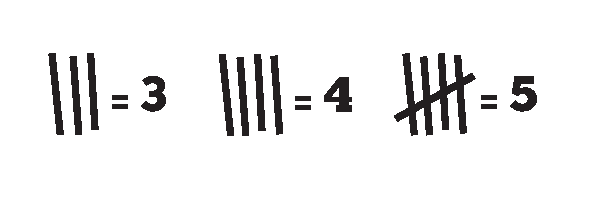
\includegraphics{pictures/Kuva1-1-tukkimiehenkirjanpito.pdf}
\end{center}

Kun käytettävissä olevien merkkien määrää lisää, suuria lukuja voi kirjoittaa lyhyempään muotoon. Tilanne on verrattavissa vaikkapa kiinan kieleen, jossa on käytössä satoja erilaisia kirjoitusmerkkejä. Merkeissä on paljon muistettavaa, mutta toisaalta kokonaisen lauseen voi kirjoittaa vain parilla kirjoitusmerkillä.



%%%ROOMALAISET LUVUT%%%%%%

\subsubsection*{Roomalaiset luvut}
Antiikin Roomassa käytössä olivat numeromerkit I, V, X, L, C, D ja M. Niiden numeroiden vastaavuudet meidän käyttämiimme lukuarvoihin ovat seuraavat:

\begin{equation*}
\rm I=1\quad
V=5\quad
X=10\quad
L=50\quad
C=100\quad
D=500\quad
M=1~000
\end{equation*}

%Huomaa, että suuri osa roomalaisista numeromerkeistä ovat jo itsessään arvoltaan niin suuria, että tarvitsemme niiden nykyilmaisuun monta merkkiä! Nollaa roomalaisissa numeroissa ei ole, ja tiettävästi tuhatta suurempia arvoja esittäviä numeromerkkejä merkkejä otettiin käyttöön vasta keskiajalla. 

Lukuja koostetaan näistä merkeistä siten, että merkit kirjoitetaan peräkkäin pääasiassa laskevassa järjestyksessä ja niiden numeroarvot lasketaan yhteen. Jos arvoltaan pienempi numeromerkki (korkeintaan yksi) edeltää suurempaa, pienempi vähennetään suuremmasta ennen yhteenlaskun jatkamista.

\begin{esimerkki}
$\text{XIV} = 10 + (5 - 1) = 14$
\end{esimerkki}

Roomalaisia numeroita käytetään usein myös nykyään merkitsemään esimerkiksi järjestystä.

\subsubsection*{Paikkajärjestelmä}

Kun numeroista koostetaan lukuja, numeroiden kirjoitusjärjestyksellä on väliä. Esimerkiksi luvut $134$ ja $413$ eivät ole sama luku; saamme eri lukuja, kun numeroita yhdistellään eri tavoin. Käsityksiä siitä, miten numeron paikka vaikuttaa luvun suuruuteen kutsutaan \emph{paikkajärjestelmiksi}.

Seuraava esimerkki selventää, miten roomalaiset muodostivat erilaisia lukuja numeromerkeistään.

\begin{esimerkki}
\ % Quick-and-dirty-fiksaus, kun ensimmäinen itemi meni ''Esimerkki.'' -tekstin perään
\begin{itemize} % https://github.com/sliedes/oppikirjamaraton-maa1/commit/e41c1cc6856f0f0b705e94b03378a1edd30f56d3
\item III$=1+1+1=3$
\item IX$=10-1=9$
\item XII$=10+1+1=12$
\item XIX$=10+(10-1)=19$
\item CDX$=500-100+10=410$
\item MDC$=1 000+500+100=1~600$
\end{itemize}
\end{esimerkki}
% Fiksattu sliedes:n kommentti: annettu kuvaus ja seuraava esimerkki itse asiassa on väärin;
% V:tä, L:ää ja D:tä ei koskaan vähennetä. Luku 1600 esitetään MDC.
% Ainakin yleisimmässä tavassa käyttää roomalaisia numeroita. 

\laatikko{Länsimaisessa traditiossa käytössämme on kymmenen numeromerkkiä: 0, 1, 2, 3, 4, 5, 6, 7, 8 ja 9. Näitä kutsutaan alkuperänsä mukaan hindu-arabialaisiksi numeroiksi.}

Kirjoittamalla näitä numeromerkkejä peräkkäin ilmaisemme lukuja.

% vanha sivulaatikko
\laatikko{Englannin kielen sana \textit{number} voi viitata sekä numeroon että lukuun. Sana \textit{digit} tarkoittaa pelkästään yhtä numeromerkkiä. Ruotsiksi luku on \textit{tal}, lukumäärä \textit{antal} ja numeroa tai lukumäärää tarkoittamatonta numeroyhdistelmää kuvaa suomen kielen tapaan sana \textit{nummer}.}

\begin{esimerkki}
Luku \[715531\] koostuu numeroista 7, 1, 5, 5, 3 ja 1.
Luku \[9\] koostuu ainoastaan vastaavasta numeromerkistä 9.
\end{esimerkki}

Luvulla on aina suuruus mutta numerolla ei. Tämän vuoksi esimerkiksi arkipäivän käsitteet postinumero ja puhelinnumero eivät ole lukuja, vaikka niissä numeroita yhdistelläänkin. Emme voi esimerkiksi sanoa, onko postinumero 00950 jollakin tapaa suurempi kuin postinumero 00900.

\subsubsection*{Lukujärjestelmät}

Järjestelmää, jolla merkitsemme lukuja kutsutaan \emph{kymmenjärjestelmäksi}. Siinä kunkin numeron paikka kertoo, kuinka monta kymmentä, sataa, tuhatta ja niin edelleen numero vastaa.

\begin{esimerkki}
Luku $562$ koostuu viidestä sadasta, kuudesta kymmenestä ja kahdesta ykkösestä, eli $562= 5 \cdot 100 + 6 \cdot 10 + 2$.

Luku $2~010,23$ koostuu kahdesta tuhannesta, yhdestä kymmenestä, kahdesta kymmenesosasta ja kolmesta sadasosasta. Desimaalimerkintöihin palataan tarkemmin Desimaaliluvut-osassa.
\end{esimerkki}

% vanha sivulaatikko
\laatikko{Kielioppihuomautuksia: 1) Tuhaterottimena käytetään välilyöntiä, ei pilkkua tai pistettä. 2) Suomessa on käytössä desimaalipilkku, ei -piste! Yhdysvaltalaiset ovat suunnitelleet laskimesi.}


Kymmenjärjestelmää kutsutaan myös \emph{desimaalijärjestelmäksi}, koska siinä hyödynnetään kymmentä eri numeromerkkiä. Muita yleisesti käytössä olevia järjestelmiä ovat 2-järjestelmä eli binäärijärjestelmä ja 16-järjestelmä eli heksadesimaalijärjestelmä, joita käytetään digitaalisen informaation tallentamiseen ja käsittelemiseen. Binäärijärjestelmässä luvun muodostavia numeromerkkejä kutsutaan biteiksi. Bitti voi olla joko päällä (1) tai pois päältä (0), ja toteutus tietokoneessa vastaa esimerkiksi sitä, että johtimessa kulkee virta (1) tai ei (0). Useampaa järjestelmää käytettäessä merkitään kantaluku luvun jälkeen alaindeksinä. Esimerkiksi luku yhdeksäntoista voidaan merkitä $19_{10}$, $10011_{2}$ tai $13_{16}$ käyttäen desimaali-, binääri- tai heksadesimaalijärjestelmää.

\begin{esimerkki}
\begin{align*}
19_{10} &= 1 \cdot 10 + 9 \\
10011_{2} &= 1 \cdot (2 \cdot 2 \cdot 2 \cdot 2) + 0 \cdot (2 \cdot 2 \cdot 2) + 0 \cdot (2 \cdot 2) + 1 \cdot 2 + 1 \\
13_{16} &= 1 \cdot 16 + 3
\end{align*}
\end{esimerkki}

Kuusitoistajärjestelmässä tarvitaan vielä kuusi uutta numeromerkkiä. Tavaksi on vakiintunut käyttää kirjainmerkkejä $\mathrm{A, B, C, D, E}$ ja $\mathrm{F}$. Ne vastaavat lukuja $10, 11, 12, 13, 14$ ja $15$. Yleisesti $n$-järjestelmässä käytetään $n$:ää kappaletta eri merkkejä, jotka merkitsevät lukuja nollasta lukuun $n-1$.

\begin{esimerkki}
$F4C_{16} = F \cdot (16 \cdot 16) + 4 \cdot 16 + C = 15 \cdot (16 \cdot 16) + 4 \cdot 16 + 12 = 3916_{10}$
\end{esimerkki}


\subsection*{Kirjaimet symboleina luvuille}

''Jos tämä on kerran matematiikkaa, niin miksi käytätte kirjaimia?'' kysyy peruskoulun alaluokkien oppilas. Lyhyt vastaus on, että näin saamme yleistettyä monia tuloksia, eikä meidän tarvitse tutkia vain erikoistapauksia.

Numeroita kuvaavat merkit ovat mielivaltaisia symboleita. Lukujakin edustamaan päädytään joskus käyttämään jotakin lyhennysmerkintää, yleensä yksittäisiä latinalaisten aakkosten kirjaimia. Kenties yleisin mielivaltaista, tuntematonta lukua edustava symboli on kirjain $x$. Kulmien suuruuksia merkitään yleensä kreikkalaisilla kirjaimilla kuten $\alpha$ (alfa), $\beta$ (beeta) ja $\gamma$ (gamma).

Jos kaksi lukua $x$ ja $2$ ovat yhtä suuret, merkitään
$x=2$. Tällainen yhtäsuuruus pätee aivan hyvin myös toisin päin: $2=x$, joten kumpikin kirjoitustapa on tilanteesta riippumatta oikein. Jos luku $y$ on pienempi kuin $z$ merkitään $y<z$, tai toisaalta $z>y$.

% vanha sivulaatikko
\laatikko{Painotekstissä kirjaimella merkityt tuntemattomat ja muuttujat kirjoitetaan \textit{kursiivilla}. Sen sijaan aina saman arvon saavat tunnetut matemaattiset vakiot kuten $\uppi$ kirjoitetaan pystyyn.} %Painotekstissä kirjaimella merkityt tuntemattomat ja muuttujat kirjoitetaan \textit{kursiivilla} ja aina saman arvon saavat, tunnetut matemaattiset vakiot kuten $\uppi$ pystyyn.

Erilaisilla luvuilla voidaan suorittaa erilaisia laskutoimituksia. Seuraavissa luvuissa esitellään ja käydään läpi lukiomatematiikassa ja mahdollisissa jatko-opinnoissa käytettäviä lukujoukkoja ja tavallisimmat laskutoimitukset.
